\chapter{Problema e Proposta}

Observando a realidade de um \textit{SmartSpace} fica claro que as informações como posição das pessoas e suas respectivas identidades são imprescindíveis para que decisões possam ser tomadas. Atualmente, a maioria das soluções encontradas para fornecer esse tipo de informação foram projetadas para funcionar em ambientes rigidamente definidos. Com isso, não seria adequado tentar incorporar soluções como estas em um ambiente com diferentes dimensões, condições de iluminação, posição dos móveis pois este se resultaria em um cenário diferente. Além disso, precisamos de uma solução que seja integrada com o middleware \textit{UbiquitOS}, o qual gerência nosso \textit{SmartSpace}.

Propomos, então, um sistema aberto de rastreamento, localização e identificação de pessoas em nosso \textit{SmartSpace} que forneça essas informações de contexto para o \textit{UbiquitOS}. Apelidamos esse sistema de TRUE, \textit{\textbf{T}racker and \textbf{R}ecognizer \textbf{U}sers in \textbf{E}nvironment}.

O sistema \textit{True} utiliza tanto imagens de cor quanto de pronfunidade. As imagens de profunidade são utilizadas no rastreamento e localização dos usuários no ambiente, e as imagens de cor são utilizadas no reconhecimento facial e no cadastro dos usuários. Então, os dispositivos presentes no ambiente devem ser capazes de fornecer esses tipos de dados a um taxa e qualidade adequada. 

Para obter esses dados do ambiente, decidimos utilizar o sensor \textit{Kinect} da Microsoft~\ref{sec:kinect}, um dispositivo bastante acessível e capaz de fornecer ao sistema imagens de cor e de profundidade sincronizadas.

O sistema \textit{True} pode ser dividido em três módulos principais:

	\begin{itemize}
		\item \textbf{Módulo de Rastreamento}: parte do sistema responsável pelo rastreamento dos usuários no ambiente.
		\item \textbf{Módulo de Reconhecimento}: parte do sistema responsável por reconhecer os usuários rastreados.
		\item \textbf{Módulo de Registro}: parte do sistema responsável pelo cadastro de novos usuários e treino do algoritmo.
	\end{itemize}

A entidade Usuário em nosso sistema possui um identificador inteiro fornecido pelo módulo de rastreamento quando é detectado, um nome fornecido pelo módulo de reconhecimento quando é reconhecido, o número de vezes que foi reconhecido e a confiança do reconhecimento.

\section{Módulo de Reconhecimento}

	O Módulo de Reconhecimento, como se deduz do próprio nome, é responsável pelo reconhecimento facial dos usuários no ambiente. Para isso, é necessário detectar a face do usuário em questão em uma imagem e depois realizar o reconhecimento da mesma em tempo real. 

	Para realizar a deteção facial foi utilizado o método \textit{Viola-Jones}~\ref{sec:viola-jones}. Um método que pode ser utilizado para construir uma abordagem de detecção facial rápida e eficaz~\cite{violajones} em tempo real. Além disso, este método é implementado pela biblioteca \textit{OpenCV} (\textit{Open Source Computer Vision}) onde bons classificadores em cascata de \textit{Haar features} são fornecidos, como por exemplo um classificador de faces frontais, utilizado nesse trabalho.

	Para realizar o reconhecimento facial foi utilizado \textit{Eigenfaces}~\ref{sec:eigenfaces}. Uma técnica bastante satisfatória quando utilizada sobre uma base de dados (faces) relativamente grande, permitindo ao sistema inferir, das imagens suas principais características e, partindo delas, realizar o reconhecimento das imagens utilizando um número bastante reduzido de cálculos~\cite{artigo-eigenface}, permitindo, assim, um reconhecimento em tempo real.

	O reconhecimento é feito em imagens de usuários que são passadas para Módulo de Rastreamento. Essa imagens são compostas somente pela região da imagem em que o usuário se encontra, como mostrado na Figura (\textbf{colocar figura aqui.}). Basicamente, o processo de reconhecimento é realizado pelas seguintes etapas e ilustrado na Figura~\ref{fig:processo-reconhecimento}:

		\begin{figure}[hbt]
			\begin{center}
				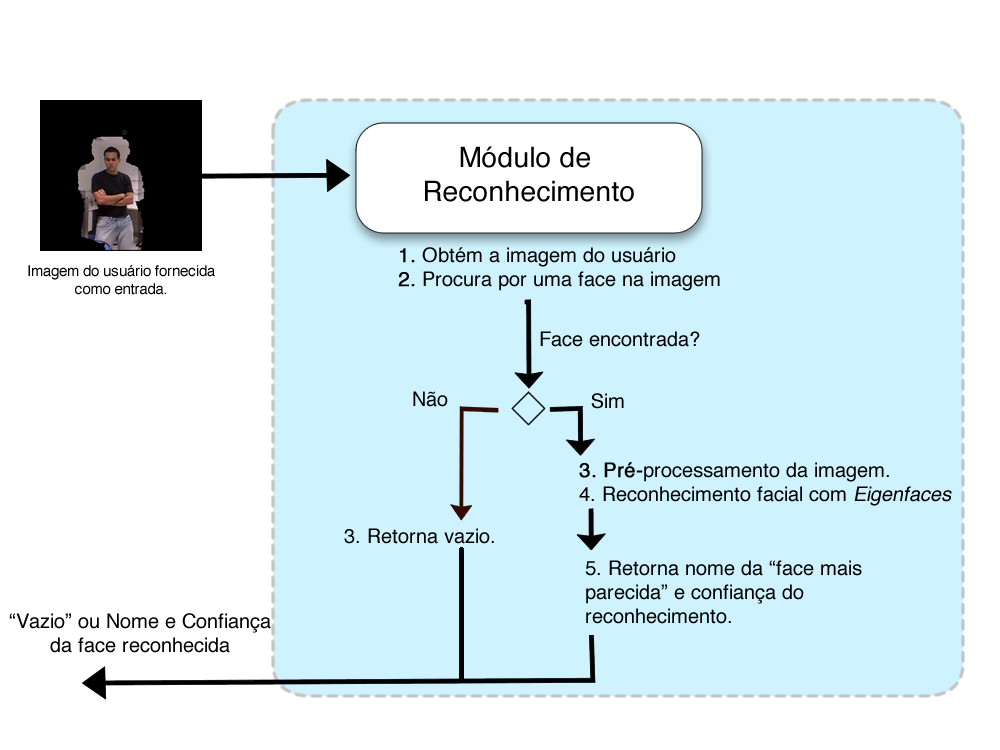
\includegraphics[scale=2.0]{figuras/4.ProblemaEProposta/reconhecimento.png}
			\end{center}
			\caption{Representação das etapas do reconhecimento facial no Módulo de Reconhecimento.}
			\label{fig:processo-reconhecimento}
		\end{figure}

		\begin{enumerate}
			\item Obtém a imagem de entrada correspondente a imagem formada somente pelo usuário cujo reconhecimento foi requisitado.
			\item Realiza detecção facial na imagem. Caso nenhuma face seja encontrada, retorna ``vazio''. Vale a pena ressaltar que no máximo uma face pode ser encontrada nesta imagem.
			\item Pré-processamento da imagem: a imagem é convertida em escala de cinza, uma nova imagem é criada recortando a região da face encontrada, a imagem, então, é redimensionada e equalizada criando assim uma padrão de tamanho, brilho e contraste nas imagens aumentando a acurácia do reconhecimento.
			\item Reconhecimento facial com \textit{Eigenfaces} é realizado.
			\item Retorna o nome da face ``mais parecida'' e a confiança do reconhecimento.
		\end{enumerate}

	O Módulo de Reconhecimento é independente dos demais módulos. Ele fica ocioso até que seja requisitado reconhecimento de um determinado usuário. No caso, o autor da requisição é o Módulo de Rastreamento. Explicaremos mais detalhadamente a relação entre os dois módulos na seção~\ref{sec:rastreamento-reconheicmento}.

\section{Módulo de Rastreamento}

	O Módulo de Rastreamento é responsável por rastrear os usuário no \textit{SmartSpace}, determinar a localização física de cada um em relação ao \textit{Kinect} e gerenciar suas identidades.

	Para realizar rastreamento e localização dos usuários foi utilizado a implementação existente na biblioteca \textit{OpenNI} (\textit{Open Natural Interaction}). Trata-se de um \textit{framework} que define \textit{APIs} para o desenvolvimento de aplicações utilizando interação natural. Utilizando as imagens de profundidade, a detecção e o rastreamento dos usuários é feita utilizando subtração de fundo~\ref{sec:deteccao-objeto} e a representação dos usuários é feita por silhuetas~\ref{sec:representacao-objeto}. 

	O rastreamento e a localização são feitas utilizando as imagens de profundidades providas pelo \textit{Kinect}, tornando-os não susceptíveis as variações nas condições de iluminação. Essas imagens de profundidade nada mais são que \textit{depth maps} (mapas de profundidade), em que cada pixel da imagem contém o valor estimado da distância em relação ao sensor. O \textit{Kinect} fornece esses dados a uma taxa de $\displaystyle 30 fps$ (\textit{frames} por segundo) com uma resolução $\displaystyle 320px$ x $\displaystyle 240px$.
	
	Com esses mapas de profundidade, a biblioteca \textit{OpenNI} consegue calcular as coodernadas $\displaystle (x,y,z)$ em relação ao \textit{Kinect} de qualquer pixel na imagem. Ou seja, se temos a representação de um usuário rastreado na imagem, conseguimos obter sua localização realativa ao \textit{Kinect}. Então, fixando a posição do mesmo no ambiente, conseguimos estimar a localização de qualquer usuário rastreado em tempo real.

\section{Relação Rastreamento e Reconhecimento}
\label{sec:rastreamento-reconheicmento}

	Até agora, mostramos como os Módulos de Rastreamento e de Reconhecimento funcionam de maneira independente, mas não mostramos como se relacionam. O Módulo de Rastreamento detém as informações sobre todos os usuários rastreados no ambiente e é responsável por requisitar reconhecimento ao Módulo de Reconhecimento.

	Basicamente, quando um novo usuário é detectado a relação entre rastreamento e reconhecimento se dá de acordo com as seguintes etapas e representado na Figura~\ref{fig:rastreamento-reconhecimento}:

		\begin{figure}[hbt]
			\begin{center}
				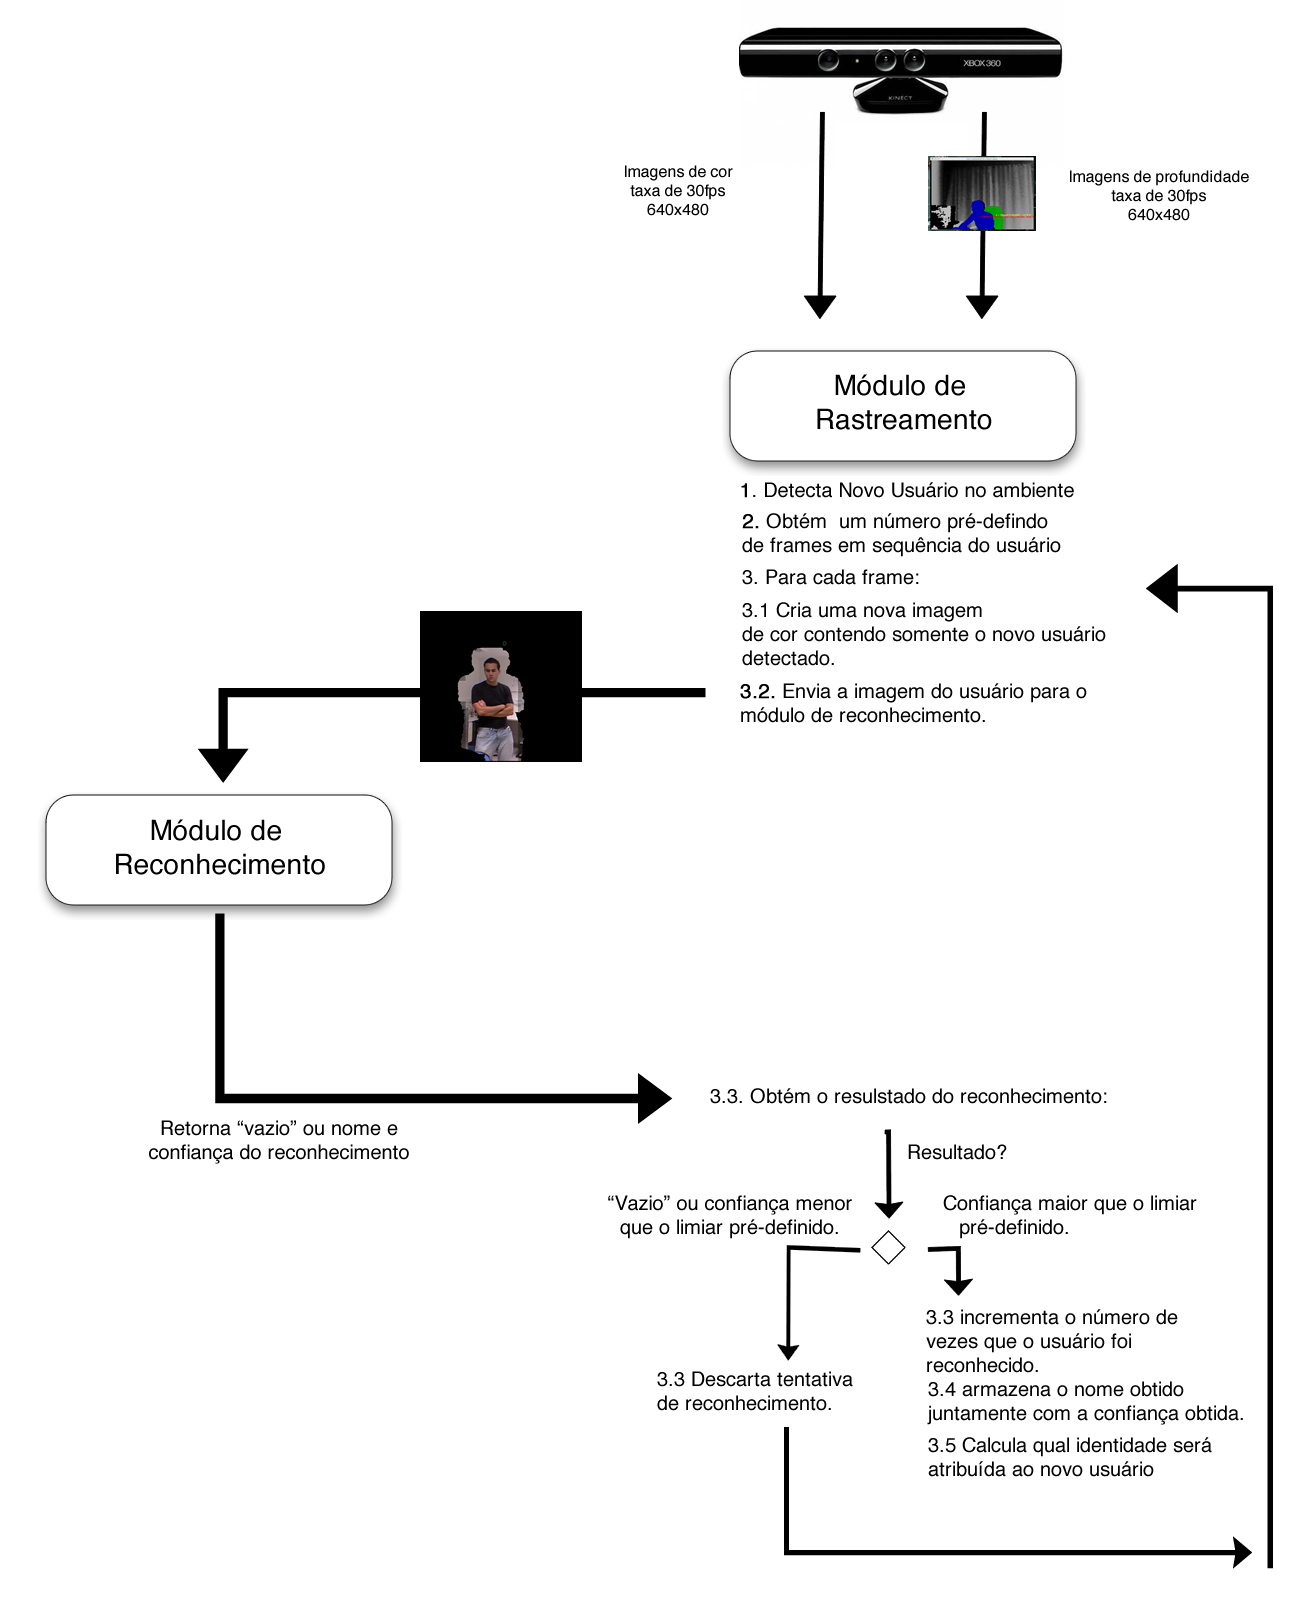
\includegraphics[scale=1.5]{figuras/4.ProblemaEProposta/esquema-tracker-reco.png}
			\end{center}
			\caption{Representação das etapas da relação que o Módulo de Rastreamento tem com o Módulo de Reconhecimento.}
			\label{fig:rastreamento-reconhecimento}
		\end{figure}
	
		\begin{enumerate}
		 	\item O Módulo de Rastreamento detecta novo usuário, e obtém um número pré-definido de imagens sucessivas do novo usuário. Para cada imagem, ele cria uma nova imagem de cor contendo somente aquele usuário, como mostrado na Figura (\textbf{colocar a figura aqui}), e a envia para o Módulo de Reconhecimento.
		 	\item Para cada imagem recebida, o Módulo de Reconhecimento tenta reconhecer o novo usuário e retorna ``vazio'' ou o nome e a confiança do reconhecimento.
		 	\item O Módulo de Rastreamento verifica se a confiança é maior que um limiar pré-definido, se for ele incrementa o contador que armazena o número de vezes que o usuário foi reconhecido, armazena o nome obtido juntamente com a confiança e calcula qual nome será atribuído ao novo usuário.
	 	\end{enumerate} 
	
	Ao invés de tentar realizar o reconhecimento somente quando novos usuários são detectados, o sistema \textit{True} continua a tentar reconhecer os usuários já reconhecidos para melhorar a confiança no reconhecimento. Essas tentativas de reconhecer novamente os usuários ocorrem em intervalos de tempo pré-definidos seguindo as mesmas etapas de quando um novo usuário é detectado. A única etapa que difere é a primeira: ao invés de obter várias imagens de um mesmo usuário, são obtidas uma imagem de cada usuário rastreado e as mesmas são enviadas ao Módulo de Reconhecimento.

	Desta maneira, o Módulo de Rastreamento consegue reunir em um só lugar todas as informações sobre os usuários rastreados, como localização corrente, nome, confiança do reconhecimento, quantas vezes o usuário foi reconhecido e quais diferentes nomes foi atribuído ao mesmo.


\section{Módulo de Registro}

	O Módulo de Registro é responsável por cadastrar novos usuários no sistema e treiná-lo para também reconhecer esse novo usuário. Basicamente, o processo de registro segue as seguintes etapas e ilustrada na Figura~\ref{fig:registro}:

		\begin{figure}[hbt]
			\begin{center}
				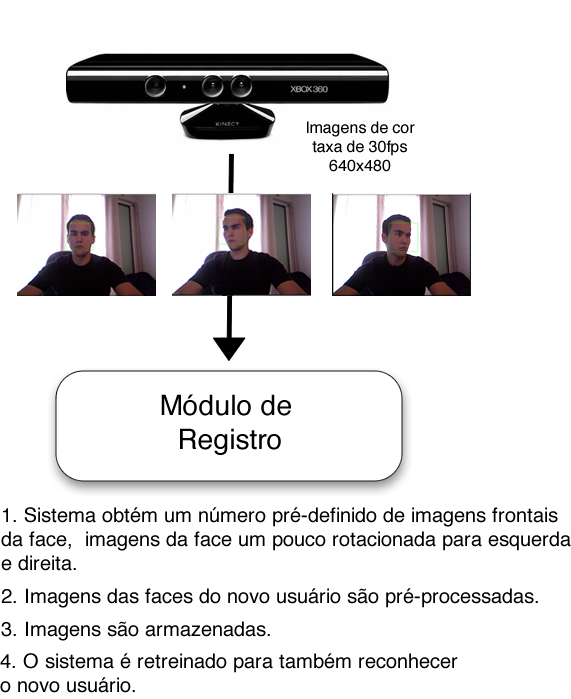
\includegraphics[scale=2.5]{figuras/4.ProblemaEProposta/registro.png}
			\end{center}
			\caption{Etapas de cadastro de um novo usuário no sistema.}
			\label{fig:registro}
		\end{figure}		

		\begin{enumerate}
			\item O novo usuário fica em uma posição fixa e frontal em relação ao \textit{Kinect}. 
			\item O sistema obtém um número pré-definido de imagens frontais do usuário.
			\item O usuário, então, rotaciona um pouco a face para a esquerda e o sistema obtém um número pré-definido de imagens do usuário. Depois, rotaciona um pouco para direita e o sistema obtém mais imagens do usuário.
			\item As imagens obtidas são processadas: as imagens são convertidas em escala de cinza, novas imagens são criadas recortando a região da face encontrada, as imagens, então, são redimensionadas e equalizadas criando assim uma padrão de tamanho, brilho e contraste nas imagens.
			\item Amarzena-se as imagens.
			\item O sistema é treinado para, também, reconhecer esse usuário.
		\end{enumerate}

	Após o treinamento, o sistema \textit{True} deve ser reiniciado para que o reconhecimento seja feito utilizando as novas informações obtidas com o treinamento.

\section{\textit{SmartSpace} Laico}

	O ambiente para o qual o sistema \textit{True} foi projetado, desenvolvido e testado foi o LAICO (\textbf{LA}boratório de sistemas \textbf{I}ntegrados e \textbf{CO}ncorrente), um laboratório do Departamento de Ciência da Computação da Universidade de Brasília. O LAICO possui dimensões de, aproximadamente,  $\displaystyle 7,67m$ x $\displaystyle 6,45m$ ilustrado pela Figura~\ref{fig:laico}.

	\begin{figure}[hbt]
			\begin{center}
				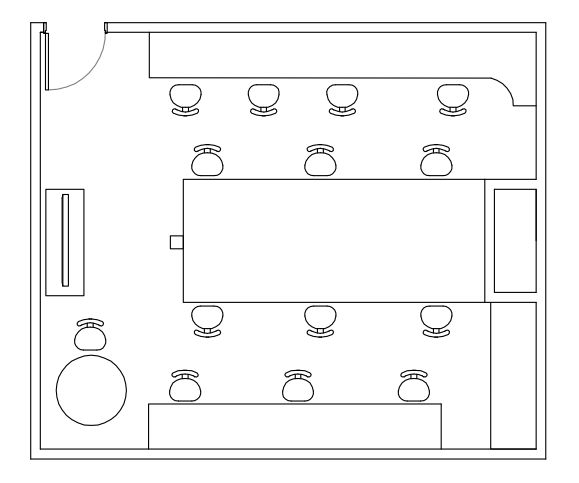
\includegraphics[scale=0.6]{figuras/4.ProblemaEProposta/laico.png}
			\end{center}
			\caption{Planta do \textit{SmartSpace} Laico.}
			\label{fig:laico}
		\end{figure}	

\section{Kinect}
\label{sec:kinect}

O Kinect, mostrado na Figura \ref{kinect}, é o nome de um projeto da Microsoft para seu console de videogame Xbox 360, que tem ainda como colaboradora a empresa Prime Sense. O projeto visa criar uma nova tecnologia capaz de permitir aos jogadores interagir com os jogos eletrônicos sem a necessidade de ter em mãos um controle(\textit{joystick}), inovando no campo da jogabilidade.

	\begin{figure}[hbt]
		\begin{center}
			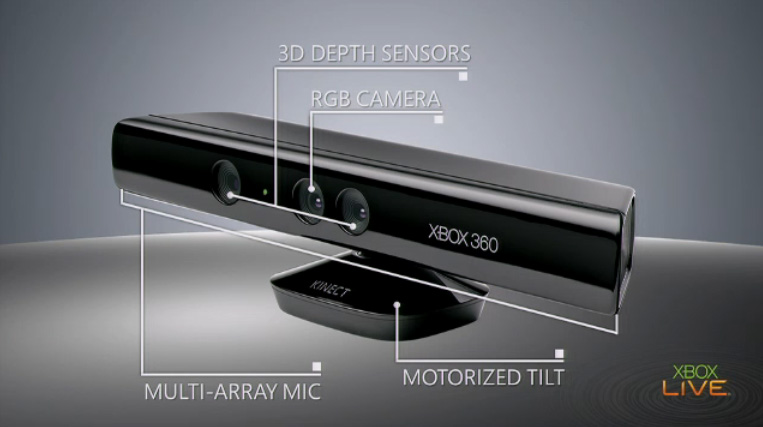
\includegraphics[scale=0.5]{figuras/2.FundamentacaoTeorica/kinect.jpg}
		\end{center}
		\caption{Sensor Kinect da Microsoft.}
		\label{kinect}
	\end{figure}

A Microsoft define o Kinect como ``jogos sem necessidade de controle e experiência de entretenimento''. Porém, vê-lo como um novo jeito de jogar é subestimar sua significância~\cite{kinect}. 

	O Kinect possui as seguintes especificações técnicas:

	\begin{itemize}
		\item Sensor
			\begin{itemize}
				\item Lentes com detecção de cores e profundidade
				\item Microfone de voz
				\item Motor de inclinação para ajuste do sensor
			\end{itemize}
		\item Campo de visão
			\begin{itemize}
				\item Campo de visão horizontal: 57 graus
				\item Campo de visão vertical: 43 graus
				\item Alcance físico da inclinação: (+/-) 27 graus
				\item Um alcance máximo de aproximadamente $\displaystyle 4.5$ metros para camêra de profundidade. 
			\end{itemize}
		\item Fluxo de Dados
			\begin{itemize}
				\item 320x240 16-bit depth a 30FPS
				\item 640x480 32-bit color a 30FPS
				\item 16-bit audio a 16 kHz
			\end{itemize}
	\end{itemize}

Basicamente, é um hardware composto por câmeras que obtém imagens de cor, som e que utiliza iluminação infra-vermelha (IR) para obter imagens de profundidade~\cite{kinect}. A Figura \ref{kinect_interno} mostra a organização interna do Kinect em alto nível.

	\begin{figure}[hbt]
		\begin{center}
			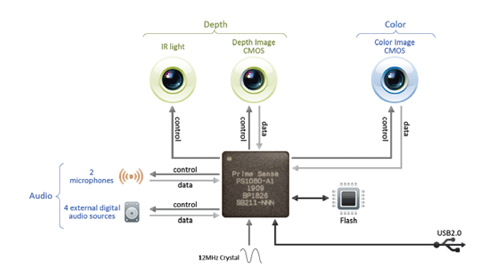
\includegraphics[scale=0.8]{figuras/2.FundamentacaoTeorica/kinect_interno.png}
		\end{center}
		\caption{Organização interna do Kinect~\cite{kinect}.}
		\label{kinect_interno}
	\end{figure}

Um chip personalizado processa os dados provindos do campo de profundidade que está correlacionado com as imagens de cor. Com isso, o software que utiliza o Kinect pode combinar cada pixel com sua profundidade. Os dados processados, são enviados para a máquina por meio de uma interface USB na forma de mapas de profundidades e imagens de cor~\cite{kinect}.

Com os dados providos pelo sensor (mapas de profundidades e imagens de cor) e pelo preço acessível, ele se torna um dispositivo adequado para tarefas como rastreamento, localização e reconhecimento facial.













